\documentclass[11pt,a4paper]{article}
\usepackage[margin=22mm]{geometry}
\usepackage[T1]{fontenc}
\usepackage{lmodern,tabularx,booktabs,hyperref,graphicx}
\usepackage[table]{xcolor}
\usepackage{titlesec,fancyhdr,enumitem}
\usepackage[most]{tcolorbox}

\definecolor{brand}{HTML}{0f5e7a}
\definecolor{accent}{HTML}{0f9d94}
\definecolor{ink}{HTML}{1a1a1a}
\definecolor{muted}{HTML}{6b6b6b}
\definecolor{rule}{HTML}{d8dce0}
\definecolor{panelbg}{HTML}{f3f7f8}

\hypersetup{colorlinks=true,urlcolor=accent,linkcolor=brand}
\setlength{\parindent}{0pt}\setlength{\parskip}{6pt}
\newcommand{\todo}[1]{\textcolor{red}{\textbf{[TODO: #1]}}}

\titleformat{\section}{\Large\bfseries\color{brand}}{\thesection}{0.6em}{}[{\color{rule}\titlerule[1pt]}]
\titleformat{\subsection}{\large\bfseries\color{ink}}{\thesubsection}{0.5em}{}
\titlespacing*{\section}{0pt}{14pt}{6pt}

\pagestyle{fancy}\fancyhf{}
\fancyhead[L]{\small\color{muted}23CSE455 --- Team B11}
\fancyhead[R]{\small\color{muted}legalSystem case study}
\fancyfoot[C]{\small\color{muted}\thepage}
\renewcommand{\headrulewidth}{0.4pt}

\begin{document}
\thispagestyle{empty}
\begin{tcolorbox}[enhanced,colback=brand,colframe=brand,arc=3pt,boxrule=0pt,
  left=16pt,right=16pt,top=14pt,bottom=14pt]
  {\color{white}\fontsize{13}{15}\selectfont 23CSE455 \textbf{Design Patterns} --- Case Study Report}\\[6pt]
  {\color{white}\LARGE\bfseries Design Pattern Identification \& Evolution}\\[2pt]
  {\color{white}\large in a Spring Boot Legal Case Management Application}
\end{tcolorbox}

\vspace{4pt}
\begin{tabularx}{\linewidth}{@{}lX@{}}
\textbf{Team} & B11\\
\textbf{Application} & \texttt{vikash0439/legalSystem} \textcolor{muted}{(commit 4e4ebb57)}\\
\textbf{Date} & 2026-10-10\\
\textbf{Repository} & \href{https://github.com/aswathymohan-amrita/23CSE455_DP_CaseStudy}{23CSE455\_DP\_CaseStudy}\\
\end{tabularx}

\vspace{6pt}
\begin{tabularx}{\linewidth}{@{}llX@{}}\toprule
\rowcolor{panelbg}\textbf{Roll number} & \textbf{Student name} & \textbf{Batch}\\\midrule
Am.sc.u4cse23237 & Lokesh & CSE\\
Am.sc.u4cse23249 & Sai Tharun & CSE\\
Am.sc.u4cse23268 & Rakshann & CSE\\
Am.sc.u4cse23311 & Nithilesh & CSE\\\bottomrule
\end{tabularx}

\begin{tcolorbox}[enhanced,colback=panelbg,colframe=accent,arc=3pt,boxrule=1pt,
  left=12pt,right=12pt,top=10pt,bottom=10pt,title=\textbf{At a glance},
  coltitle=white,colbacktitle=accent,fonttitle=\bfseries]
\begin{tabularx}{\linewidth}{@{}Xr@{}}
Confirmed pattern types (baseline) & \textbf{5}\\
Recorded instances (incl. 1 idiom, 1 uncertain) & \textbf{7}\\
Changes implemented (CH01--CH03) + refactor & \textbf{3 + 1}\\
Cross-language implementations (4 patterns $\times$ 4 langs) & \textbf{16}\\
Part~2 unit tests (\texttt{mvn test}) & \textbf{7 pass / 0 fail}\\
Application boots with changes (MySQL) & \textbf{yes}\\
\end{tabularx}
\end{tcolorbox}

\section{Application and architecture}
\textbf{Original source:} \url{https://github.com/vikash0439/legalSystem}; baseline commit \texttt{4e4ebb574d6730614855899e032fd5a79b04da63} (2023-03-18); accessed 2026-10-10. \textbf{License:} the repository contains no LICENSE file; the code is therefore used for non-commercial academic study only, under the course's fair-use scope, with the author credited.\par
\textbf{Environment:} Java 8 (repo targets JVM 1.8.0\_171); Spring Boot 2.4.0; Spring Security; Spring Data JPA; Hibernate 5.3; MySQL; JSP 2.2; Maven (mvnw wrapper). Cross-language snippets measured on the submission machine (Apple~Silicon macOS): OpenJDK~11.0.32, CPython~3.9.6, Node.js~25.9.0, Apple~clang~21.0.0.\par
\textbf{Scope:} Inspected \texttt{rest/}, \texttt{main/}, \texttt{service/}, \texttt{repository/}, \texttt{modal/}, \texttt{config/}, \texttt{mail/}, and \texttt{LegalAppApplication.java}. Excluded JSP views, static assets, \texttt{bin/}, \texttt{DB\_backup/}, \texttt{.recommenders/} (not application logic).\par
\textbf{Architecture:} Layered Spring MVC --- Controller ($\rightarrow$) Service ($\rightarrow$) Repository ($\rightarrow$) MySQL, with a scheduler (\texttt{@EnableScheduling}) driving \texttt{EmailServiceImpl} for reminders (editable source: \texttt{Part1/diagrams/src/architecture.puml}).\par
\begin{center}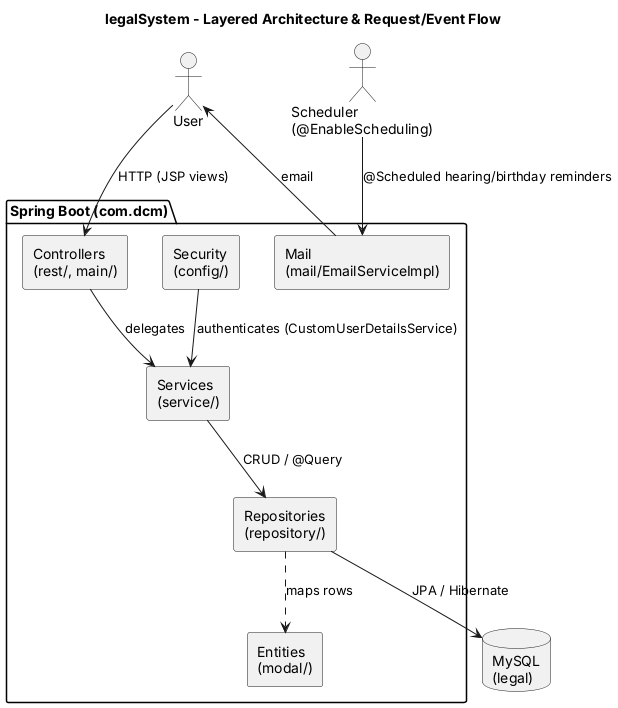
\includegraphics[width=0.72\linewidth]{Part1/diagrams/img/architecture.png}\end{center}
\textbf{Run instructions:} \texttt{./mvnw spring-boot:run} (Maven wrapper included), serving JSP views on Tomcat; it requires a local MySQL database named \texttt{legal} configured in \texttt{application.properties}. Note the baseline ships a \emph{stubbed} password encoder (plaintext) --- fixed in CH03. With the Part~2 changes applied, the application was booted against MySQL and the login page served at \texttt{http://localhost:8080/login} (HTTP~200); the live page is shown below. Startup log: \texttt{test\_result/app\_startup.log}; screenshot: \texttt{test\_result/app\_screenshot.png}.\par
\begin{center}\fbox{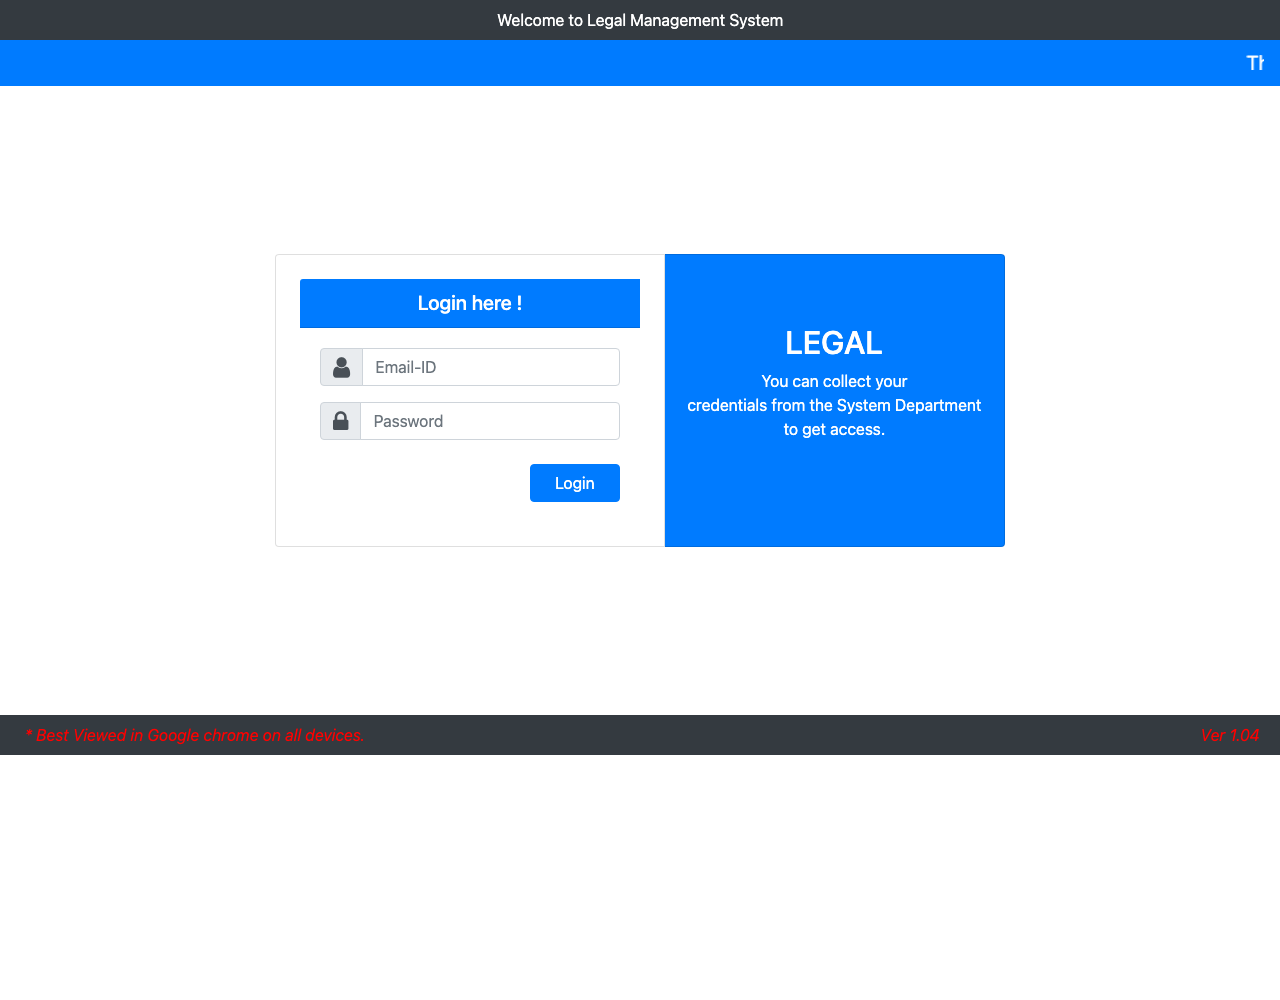
\includegraphics[width=0.78\linewidth]{test_result/app_screenshot.png}}\\[2pt]{\small\color{muted}Live \texttt{/login} page served by the running application (MySQL-backed).}\end{center}

\section{Part 1 Pattern discovery}
\textbf{Method:} Each candidate was located by reading the Java source and confirmed against the exact class/interface/method and its \texttt{file:line}. A class name, annotation, or LLM assertion alone was treated as insufficient; every row in \texttt{data/patterns.csv} is backed by a cited line (see \texttt{Part1/evidence/verification\_notes.md}).

\subsection{Totals at the baseline}
\textbf{Confirmed pattern types:} 5 (Adapter, Template Method, Strategy, Repository, Copy Constructor).\par
\textbf{Confirmed pattern instances:} 7 total rows (5 confirmed + 1 framework idiom + 1 uncertain).\par
\textbf{Concrete participant classes:} 10 app-authored concrete classes play pattern roles (CustomUserDetails, Users, CustomUserDetailsService, SecurityConfiguration, the anonymous encoder, CaseRepository (representative of 15), Case, CaseService, EmailServiceImpl, LegalAppApplication). Enumerated in \texttt{Part1/evidence/counts.md}.\par
\textbf{Unique participant symbols:} 14 distinct symbols (the 10 above + 4 framework interfaces: UserDetails, WebSecurityConfigurerAdapter, PasswordEncoder, CrudRepository). The 15 repository interfaces share one role and are counted once.\par
\textbf{Rejected and uncertain candidates:} Uncertain: 1 (Observer). Rejected: 3 (Singleton --- Spring bean scope is not GoF \texttt{getInstance}; Factory; Builder). Framework idiom: 1 (Dependency Injection).\par

\subsection{Pattern inventory}
\begin{tabularx}{\linewidth}{@{}lXll@{}}\toprule
Pattern type & Instance names & Instances & Concrete classes\\\midrule
Adapter & User-to-Security Adapter & 1 & 1\\
Template Method & Security Configuration Callback & 1 & 1\\
Strategy & Password Encoding Strategy & 1 & 1\\
Repository & Case Persistence Repository & 1 & 15 (counted as 1 type)\\
Copy Constructor & Users Defensive Copy & 1 & 1\\
Dependency Injection (idiom) & Service-Repository Wiring & 1 & n/a\\
Observer (uncertain) & Hearing/Reminder Notification & 1 & --\\\bottomrule
\end{tabularx}

\subsection{One record for each pattern instance}

\textbf{(1) Adapter --- User-to-Security Adapter.} Category: Structural (GoF). Purpose: adapt the app's \texttt{Users} entity to Spring Security's \texttt{UserDetails} so app users can authenticate (application-level).\par
\begin{tabularx}{\linewidth}{@{}lXX@{}}\toprule
Role & Actual symbol & File:lines\\\midrule
Target & \texttt{UserDetails} (Spring) & (framework)\\
Adaptee & \texttt{Users} & modal/Users.java:8--113\\
Adapter & \texttt{CustomUserDetails} & modal/CustomUserDetails.java:10--66\\
Client & \texttt{CustomUserDetailsService.loadUserByUsername} & service/CustomUserDetailsService.java:24--32\\\bottomrule
\end{tabularx}
Evidence: \texttt{CustomUserDetails extends Users implements UserDetails}; \texttt{getAuthorities()} (line 23) maps roles to \texttt{SimpleGrantedAuthority}; client maps via \texttt{CustomUserDetails::new} (line 31). Verification: \textbf{confirmed}.\par
\begin{center}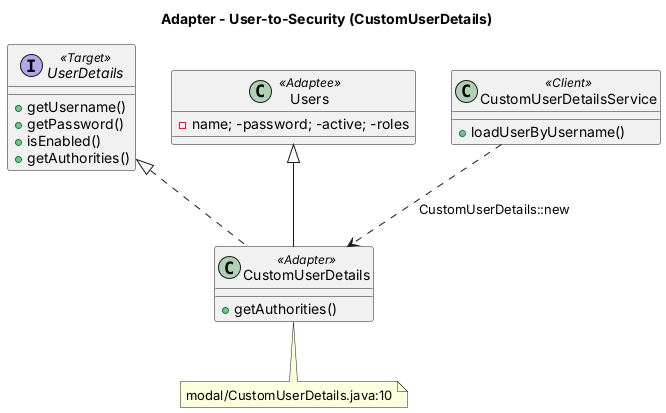
\includegraphics[width=0.78\linewidth]{Part1/diagrams/img/adapter.png}\end{center}

\textbf{(2) Template Method --- Security Configuration Callback.} Category: Behavioral (GoF). Purpose: framework fixes the security-setup algorithm; the app fills variable steps (framework idiom realised as Template Method).\par
\begin{tabularx}{\linewidth}{@{}lXX@{}}\toprule
Role & Actual symbol & File:lines\\\midrule
AbstractClass & \texttt{WebSecurityConfigurerAdapter} & (framework)\\
ConcreteClass & \texttt{SecurityConfiguration} & config/SecurityConfiguration.java:23\\
PrimitiveOp & \texttt{configure(AuthenticationManagerBuilder)} & config/SecurityConfiguration.java:29--33\\
PrimitiveOp & \texttt{configure(HttpSecurity)} & config/SecurityConfiguration.java:35--54\\\bottomrule
\end{tabularx}
Evidence: both \texttt{configure(...)} hooks are overridden and invoked by the framework inside its own flow. Verification: \textbf{confirmed}.\par
\begin{center}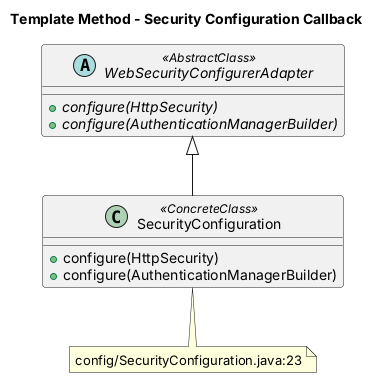
\includegraphics[width=0.6\linewidth]{Part1/diagrams/img/template_method.png}\end{center}

\textbf{(3) Strategy --- Password Encoding Strategy.} Category: Behavioral (GoF). Purpose: a pluggable password algorithm injected into the authentication context.\par
\begin{tabularx}{\linewidth}{@{}lXX@{}}\toprule
Role & Actual symbol & File:lines\\\midrule
Strategy & \texttt{PasswordEncoder} & config/SecurityConfiguration.java:12\\
ConcreteStrategy & anonymous \texttt{BCryptPasswordEncoder} subclass & config/SecurityConfiguration.java:57--77\\
Context & \texttt{auth.passwordEncoder(...)} & config/SecurityConfiguration.java:31\\\bottomrule
\end{tabularx}
Evidence: \texttt{getPasswordEncoder()} returns a \texttt{PasswordEncoder} passed into the auth builder. \textbf{Note:} the concrete strategy is \emph{stubbed} --- \texttt{encode}/\texttt{matches} compare plaintext, so the structure is present but insecure (target of CH03). Verification: \textbf{confirmed} (structure); implementation flagged.\par
\begin{center}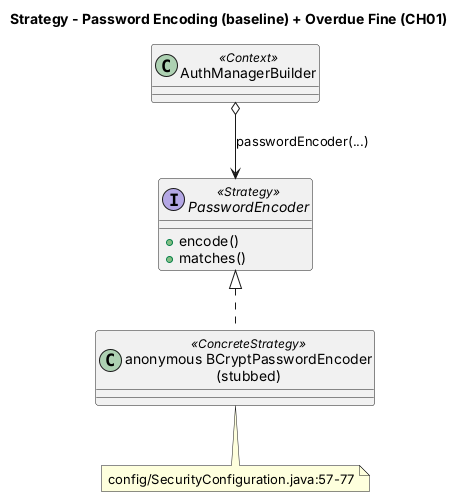
\includegraphics[width=0.6\linewidth]{Part1/diagrams/img/strategy.png}\end{center}

\textbf{(4) Repository --- Case Persistence Repository.} Category: Architecture / DDD idiom. Purpose: abstract data access behind a collection-like interface; Spring Data generates the implementation.\par
\begin{tabularx}{\linewidth}{@{}lXX@{}}\toprule
Role & Actual symbol & File:lines\\\midrule
Repository (abstract) & \texttt{CrudRepository}/\texttt{JpaRepository} & (Spring Data)\\
ConcreteRepository & generated proxy & (runtime)\\
Domain entity + queries & \texttt{CaseRepository} & repository/CaseRepository.java:12--26\\\bottomrule
\end{tabularx}
Evidence: \texttt{CaseRepository extends CrudRepository<Case,Integer>} with derived + \texttt{@Query} finders; 15 such interfaces exist, counted as \textbf{one} instance type. Verification: \textbf{confirmed}.\par
\begin{center}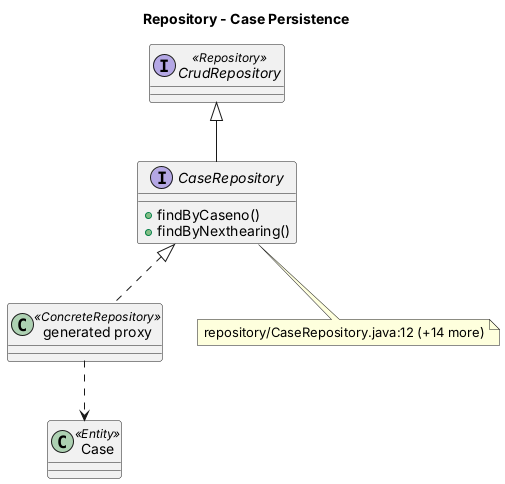
\includegraphics[width=0.6\linewidth]{Part1/diagrams/img/repository.png}\end{center}

\textbf{(5) Copy Constructor --- Users Defensive Copy.} Category: Creational idiom. Purpose: build a new \texttt{Users} from an existing one.\par
\begin{tabularx}{\linewidth}{@{}lXX@{}}\toprule
Role & Actual symbol & File:lines\\\midrule
Source + copy & \texttt{Users(Users users)} & modal/Users.java:38--47\\
User of copy & \texttt{CustomUserDetails} \texttt{super(users)} & modal/CustomUserDetails.java:16\\\bottomrule
\end{tabularx}
Evidence: copies every field; used by the Adapter's constructor. Verification: \textbf{confirmed} (idiom, not GoF Prototype).\par
\begin{center}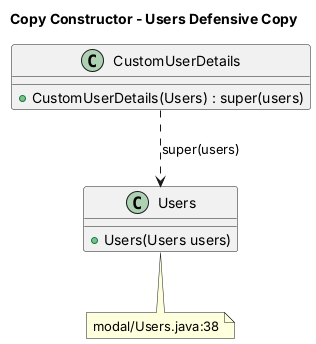
\includegraphics[width=0.55\linewidth]{Part1/diagrams/img/copy_constructor.png}\end{center}

\textbf{(6) Dependency Injection --- Service-Repository Wiring.} Category: framework idiom (IoC). Participants: Spring container (injector), \texttt{CaseService}, \texttt{CaseRepository} (constructor-injected, service/CaseService.java:18--21). Verification: \textbf{confirmed as framework idiom}, not hand-written GoF.\par
\begin{center}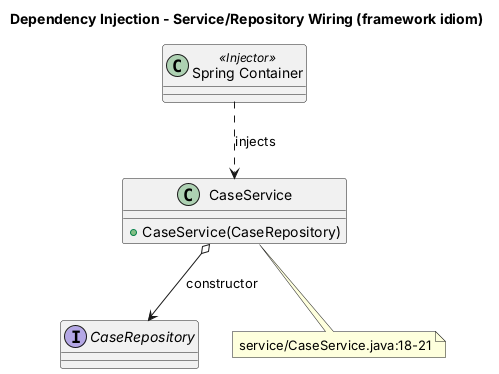
\includegraphics[width=0.6\linewidth]{Part1/diagrams/img/dependency_injection.png}\end{center}

\textbf{(7) Observer --- Hearing/Reminder Notification.} Category: Behavioral (GoF) --- \textbf{UNCERTAIN}. Participants: \texttt{@Scheduled} trigger (LegalAppApplication.java:25,45,81,88) $\rightarrow$ \texttt{EmailServiceImpl}. Evidence: timer-driven broadcast of hearing/reminder/birthday notifications. \textbf{Why uncertain:} no Subject maintains a list of registered Observers --- it is scheduler-triggered, not subject-observer registration. Recorded as uncertain; CH02 evolves it into a true Observer.\par
\begin{center}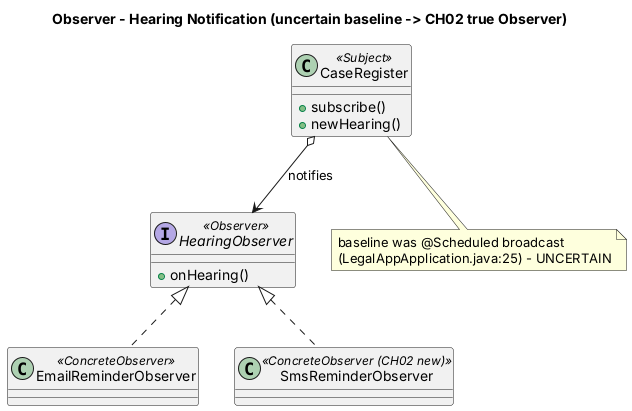
\includegraphics[width=0.72\linewidth]{Part1/diagrams/img/observer.png}\end{center}

\section{Part 2 Evolution and refactoring}
Three changes implemented: CH01 (new late-fee Strategy), CH02 (SMS channel, extends Observer), CH03 (replace stubbed encoder with real BCrypt --- refactor). The three changes were applied to the baseline clone and committed (\texttt{baseline 4e4ebb57} $\rightarrow$ \texttt{after c31ce44}), and each ships a JUnit~5 test. Running \texttt{mvn test} on the three test classes gave \textbf{BUILD SUCCESS --- Tests run: 7, Failures: 0, Errors: 0} (\texttt{FineServiceTest} 3, \texttt{CaseRegisterTest} 2, \texttt{PasswordEncoderTest} 2; log in \texttt{test\_result/mvn\_test.log}). CH03 is a unified diff against the real baseline file (\texttt{Change3/change3.diff}). With the changes applied, the full application boots successfully against MySQL --- \texttt{Started LegalAppApplication} with Hibernate creating the schema (\texttt{test\_result/app\_startup.log}).\par
\textbf{Integration findings (honest).} Two real issues surfaced only when the code was compiled and run, which is the point of Part~2: (i)~CH01 first failed context startup with \texttt{NoUniqueBeanDefinitionException} --- two \texttt{FinePolicy} beans (\texttt{regularFine}, \texttt{advocateFine}) with no way to choose; resolved by marking \texttt{RegularFine} \texttt{@Primary} as the default injected strategy (callers still switch via \texttt{setPolicy}). (ii)~The baseline's own test \texttt{LegalAppApplicationTests} is JUnit~4, but Spring~Boot~2.4 dropped the JUnit~Vintage engine, so it no longer compiles; the three new tests are JUnit~5 and pass. Both are recorded in \texttt{test\_result/ENVIRONMENT\_NOTES.md}.\par
\textbf{Pattern effects summary:} CH01 \emph{newly\_introduced} Overdue Fine Strategy (Password Strategy preserved); CH02 \emph{modified} the Hearing Notification into a real Observer; CH03 \emph{modified} the Password Strategy's concrete class (structure preserved).\par

\subsection{Updated pattern counts}
Per-snapshot totals (full rows in \texttt{data/patterns\_evolution.csv}; instance names preserved for continuing collaborations):\par
\begin{tabularx}{\linewidth}{@{}Xcccc@{}}\toprule
Snapshot & Confirmed types & Instances & Uncertain & Newly introduced\\\midrule
baseline & 5 & 7 & 1 (Observer) & --\\
after CH01 & 5 & 8 & 1 & +1 (Overdue Fine Strategy)\\
after CH02 & 6 & 8 & 0 & -- (Observer becomes confirmed)\\
after CH03 & 6 & 8 & 0 & -- (Strategy concrete class replaced)\\\bottomrule
\end{tabularx}
\textbf{Interpretation:} The most informative outcome is qualitative, not a line count. CH01 adds a second Strategy collaboration cleanly because the pattern was already present, demonstrating the Open/Closed benefit --- a new fee rule needs no change to callers. CH02 is the key design win: it converts the baseline scheduler-driven broadcast (recorded \emph{uncertain}) into a genuine subject-maintains-observers Observer, so adding the SMS channel touches no existing code; the trade-off is a small increase in classes and indirection. CH03 corrects a security defect by replacing the concrete strategy while leaving the Strategy structure and wiring intact --- proving the pattern's substitutability. Fewer or more LOC alone does not prove better design; here the gains are decoupling (CH01, CH02) and correctness (CH03). Remaining limitation: the app still lacks tests around these paths, so behaviour preservation rests on the added JUnit cases.\par

\section{Part 3 Cross-language comparison}
\textbf{Selected instances:} Strategy (late-fee policy), Adapter (user-to-security), Template Method (case report), Observer (hearing notification) --- one representative per confirmed type (Observer in its canonical subject-observer form).\par
\textbf{Common specifications:} each pattern has fixed inputs and expected outputs; all four languages must print identical lines (evidence: \texttt{test\_result/part3\_output.txt}).\par
\textbf{Implementations:} \texttt{Part3/<pattern>/\{java,python,javascript,cpp\}} with per-folder run commands.\par
\textbf{Actual results:} all 16 implementations compiled and ran; 8/8 shared cases pass per language (identical output verified).\par
\begin{center}
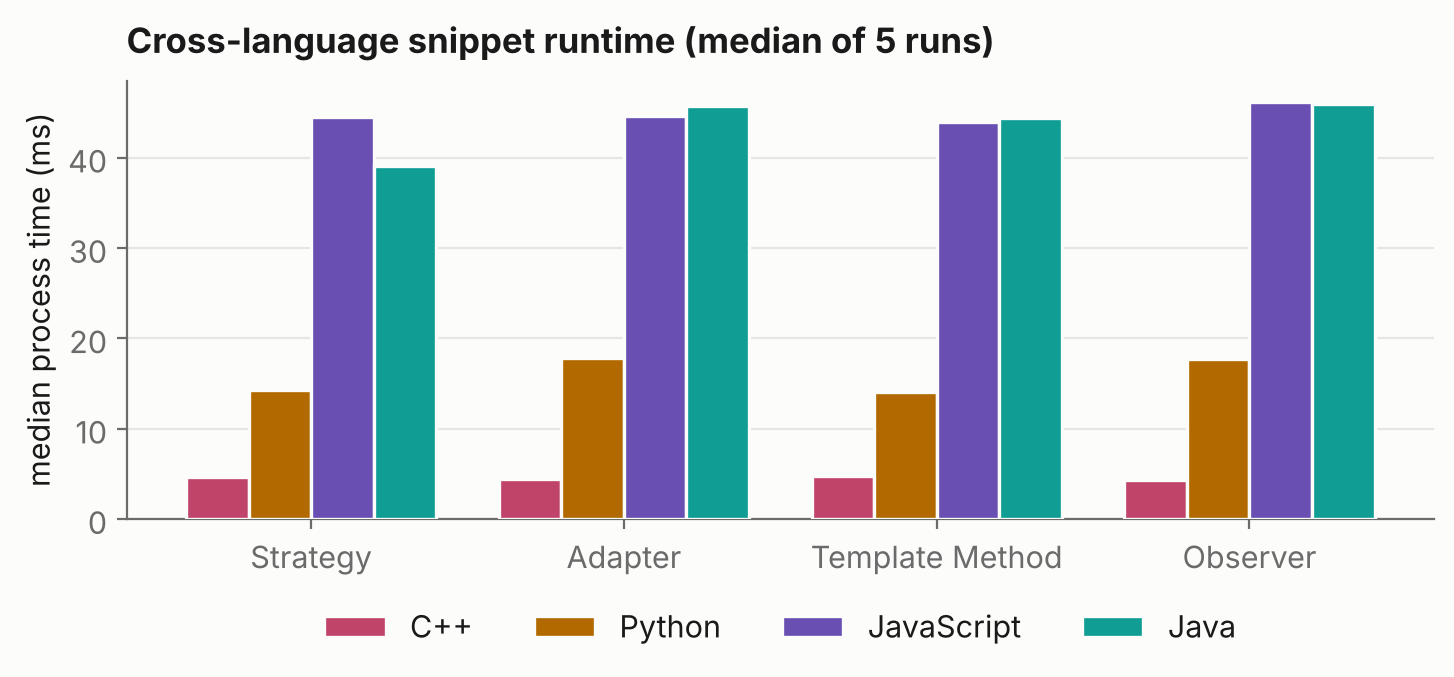
\includegraphics[width=0.92\linewidth]{Part3/charts_timing.png}\\[6pt]
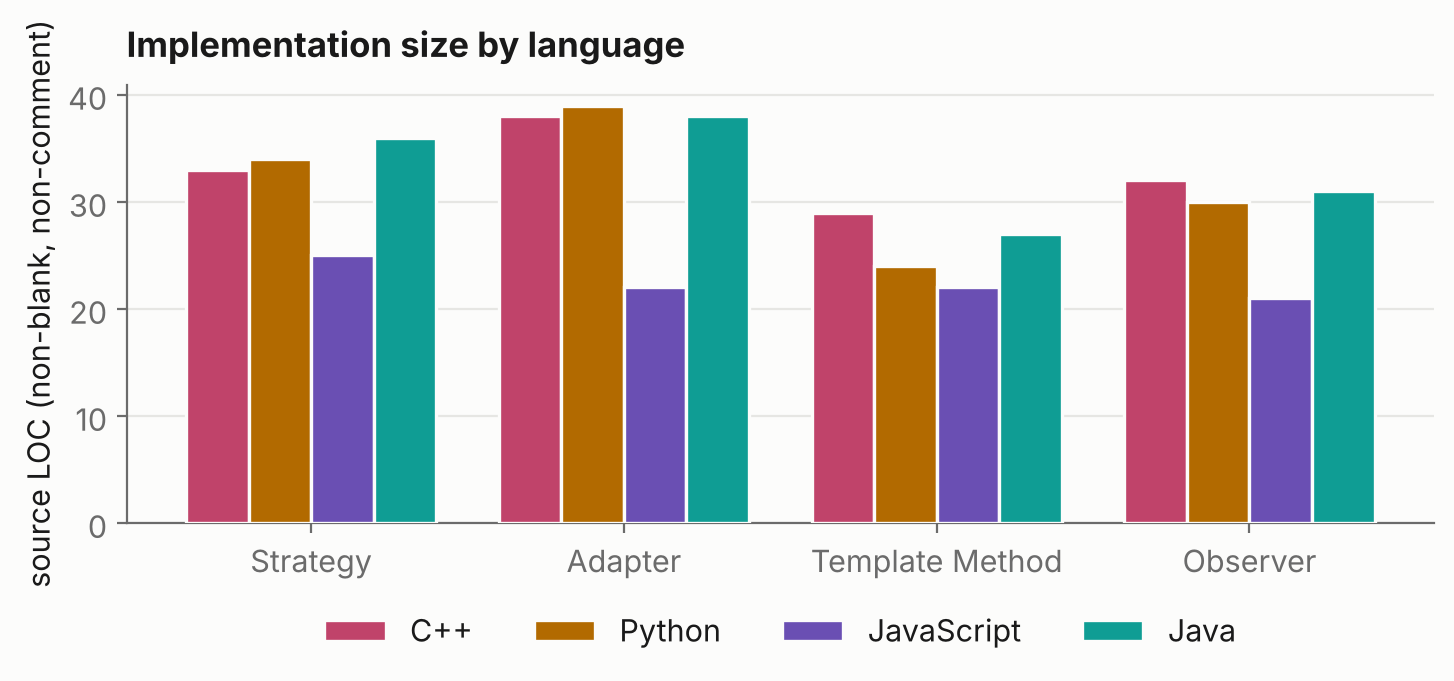
\includegraphics[width=0.92\linewidth]{Part3/charts_loc.png}
\end{center}
\textbf{Static and dynamic comparison:} recorded in \texttt{data/cross\_language.csv} --- source LOC, max function cyclomatic complexity (measured with \textbf{lizard}), runtime/compiler, test command/result, and the median of 5 timed runs (compile once, 1 warmup, 5 measured). Measured on the submission machine (Apple~Silicon macOS; OpenJDK~11.0.32, CPython~3.9.6, Node.js~25.9.0, Apple~clang~21): C++ $\approx$4.5\,ms $<$ Python $\approx$15\,ms $<$ Java $\approx$44\,ms $\approx$ JavaScript $\approx$45\,ms. C++ is an order of magnitude faster (native, no VM startup); Python's interpreter starts quickly; Java and JavaScript are close here, both paying VM/runtime startup that dwarfs the trivial workload. Full per-case figures in \texttt{data/cross\_language.csv}; the protocol is compile once, 1 warmup, 5 measured runs, median.\par
\textbf{Comparison:} C++ uses abstract base + virtual dispatch; Java uses interfaces; Python uses ABCs (duck typing optional); JavaScript uses prototype classes with no interface keyword. \par
\textbf{Technology discussion:} The measured ordering (C++ $\approx$4.5\,ms $<$ Python $\approx$15\,ms $<$ Java $\approx$44\,ms $\approx$ JavaScript $\approx$45\,ms) reflects process-startup cost far more than the patterns themselves, since each snippet does trivial work. C++ compiles to native code and starts almost instantly; CPython and Node start an interpreter/VM; the JVM pays the largest fixed cost to bootstrap and JIT-warm before \texttt{main} runs, which dominates such short programs (a well-known JVM ``startup problem''). For the dispatch the patterns rely on, all four are comparable: Java/C++ resolve virtual calls through a vtable, while Python and JavaScript dispatch dynamically at runtime. The design lesson for the course: the same GoF structure is expressible in every language, but the language's execution model --- compiled vs interpreted, static vs dynamic dispatch --- sets the performance floor, not the pattern.\par

\section{LLM records and human verification}
\textbf{Run and model:} Claude Opus 4.8, 2026-10-10, used for Part 1 discovery and Part 3 cross-language drafting. \textbf{Inputs and outputs:} prompts/inputs/outputs saved under \texttt{Part1/llm/} and \texttt{Part3/llm/}; baseline commit recorded. \textbf{Claims and evaluation:} Part 1 --- \emph{partially correct}: pattern list verified against source, Observer downgraded to uncertain by the team, DI/Repository relabelled as framework idioms (see \texttt{Part1/evidence/verification\_notes.md}). Part 3 --- \emph{correct}: all implementations compiled and produced identical output, metrics measured. \textbf{Generated code:} the Part 3 snippets were generated then compiled/run/tested by the team. See \texttt{data/llm.csv}.\par

\section{Findings, contributions and references}
\textbf{Findings:} the baseline app contains 5 confirmed pattern types (7 recorded instances incl. 1 idiom, 1 uncertain); the Strategy is structurally present but its concrete implementation is an insecure stub; the notification mechanism is scheduler-driven rather than a true Observer until CH02. \par
\textbf{Contributions:}\par
\begin{tabularx}{\linewidth}{@{}llX@{}}\toprule
Roll number & Name & Contribution\\\midrule
Am.sc.u4cse23237 & Lokesh & Adapter (Part1 record + Part3 4-lang); architecture diagram; CSV merge\\
Am.sc.u4cse23249 & Sai Tharun & Template Method (Part1 + Part3); CH03 refactor; evolution CSV\\
Am.sc.u4cse23268 & Rakshann & Strategy (Part1 + Part3); CH01; report assembly + final PDF\\
Am.sc.u4cse23311 & Nithilesh & Observer (Part1 + Part3); CH02; README; llm.csv; repo setup\\\bottomrule
\end{tabularx}
\textbf{(Link each row to its commits in the team repo before final submission.)}\par
\textbf{References:}\par
\begin{enumerate}
\item vikash0439, \emph{legalSystem} (Spring Boot legal case management), GitHub, commit \texttt{4e4ebb57}, accessed 2026-10-10. \url{https://github.com/vikash0439/legalSystem}
\item E. Gamma, R. Helm, R. Johnson, J. Vlissides, \emph{Design Patterns: Elements of Reusable Object-Oriented Software}, Addison-Wesley, 1994.
\item Spring Security Reference Documentation, \url{https://docs.spring.io/spring-security/reference/}
\item Spring Data JPA Reference Documentation, \url{https://docs.spring.io/spring-data/jpa/reference/}
\item Tool versions (submission machine): OpenJDK 11.0.32; CPython 3.9.6; Node.js 25.9.0; Apple clang 21.0.0; lizard (cyclomatic complexity); PlantUML (diagrams).
\end{enumerate}

\section{Team folder and datasets}
\begin{verbatim}
B11/
  README.md  B11_Report.tex  B11_Final_Report.pdf
  data/   patterns.csv  pattern_counts.csv  patterns_evolution.csv
          cross_language.csv  llm.csv
  code/   (baseline source snapshot at the recorded commit)
  test_result/   part3_output.txt  charts_*.png  (+ repo screenshots)
  Part1/  diagrams/  evidence/  llm/
  Part2/  code/changes/{Change1,Change2,Change3}/ (src + test + diff)  diagrams/  llm/
  Part3/  strategy/ adapter/ template_method/ observer/  charts_*.png  llm/  measure.py
\end{verbatim}

\end{document}
